\documentclass[a4paper, 11pt]{article}
\usepackage{geometry}
\geometry{letterpaper, margin=1in}
\usepackage{graphicx}
\graphicspath{ {images/} }

\usepackage{amsmath}
\usepackage{amssymb}  
\usepackage{amsthm}
\usepackage{ulem}

\usepackage{enumitem}


\usepackage{pdfpages} % for including full pdf pages

\usepackage{empheq}

\usepackage{listings}


%format to allow bolded theorems, corollaries, etc...
\newtheorem*{theorem}{Theorem}
\newtheorem*{corollary}{Corollary}
\newtheorem*{lemma}{Lemma}
\newtheorem*{definition}{Definition}
\newtheorem*{Example}{Example} 
\newtheorem*{Remark}{Remark}

% stop typing \mathbb a thousand times 
\newcommand{\R}{\mathbb{R}}
\newcommand{\C}{\mathbb{C}}
\newcommand{\F}{\mathbb{F}}
\newcommand{\E}{\mathbb{E}}
\newcommand{\sphere}{\mathbb{S}}

% commands for bra-ket notation
\newcommand{\bra}[1]{\ensuremath{\left\langle#1\right|}}
\newcommand{\ket}[1]{\ensuremath{\left|#1\right\rangle}}
\newcommand{\bracket}[2]{\ensuremath{\left\langle #1 \middle| #2 \right\rangle}}
\newcommand{\matrixel}[3]{\ensuremath{\left\langle #1 \middle| #2 \middle| #3 \right\rangle}}
\newcommand{\expectation}[1]{\ensuremath{\left\langle #1 \right\rangle}}

% vector stuff
\newcommand{\basis}[1]{\hat{\mathbf{e}}_#1}
\newcommand{\unit}[1]{\hat{\boldsymbol{#1}}}
\newcommand{\bvec}[1]{\vec{\boldsymbol{#1}}}


% change margins for solution
\newenvironment{solution}{%
	\begin{list}{}{%
			\setlength{\topsep}{0pt}%
			\setlength{\leftmargin}{0.5cm}%
			\setlength{\rightmargin}{0.5cm}%
			\setlength{\listparindent}{\parindent}%
			\setlength{\itemindent}{\parindent}%
			\setlength{\parsep}{\parskip}%
		}%
		\item[]}{\end{list}}



\begin{document}
\noindent
\large\textbf{Assignment 3: Design} \hfill \textbf{John Waczak} \\
\normalsize CS 162 \hfill  Date: \today 
\par\noindent\rule{\textwidth}{0.4pt} \\\\



\section*{Understanding the problem}

\textit{In your own words, explain what YOU think the problem is asking you to
  do.  Document your uncertainties about the problem and anything else that you
  feel was unclear or vague}\\

This problem is asking us to design a zoo tycoon type simulation which will
allow the ``owner'' of the zoo to purchase animals, purchase food, earn revenue,
each week. The owner begins with no animals and $\$100,000$ dollars and the
simulation finishes if the owner runs out of money. 

\section*{Devising a plane/design}

\textit{Provide an algorithm/pseudo code to help solve the problem. In addition,
  draw pictures/flow charts to help you devise your plan, as well as any other
  design decisions you make, such as how to manage your time, how to decompose
  the problem, where to start first, etc. }\\ 

See flowchart on next page

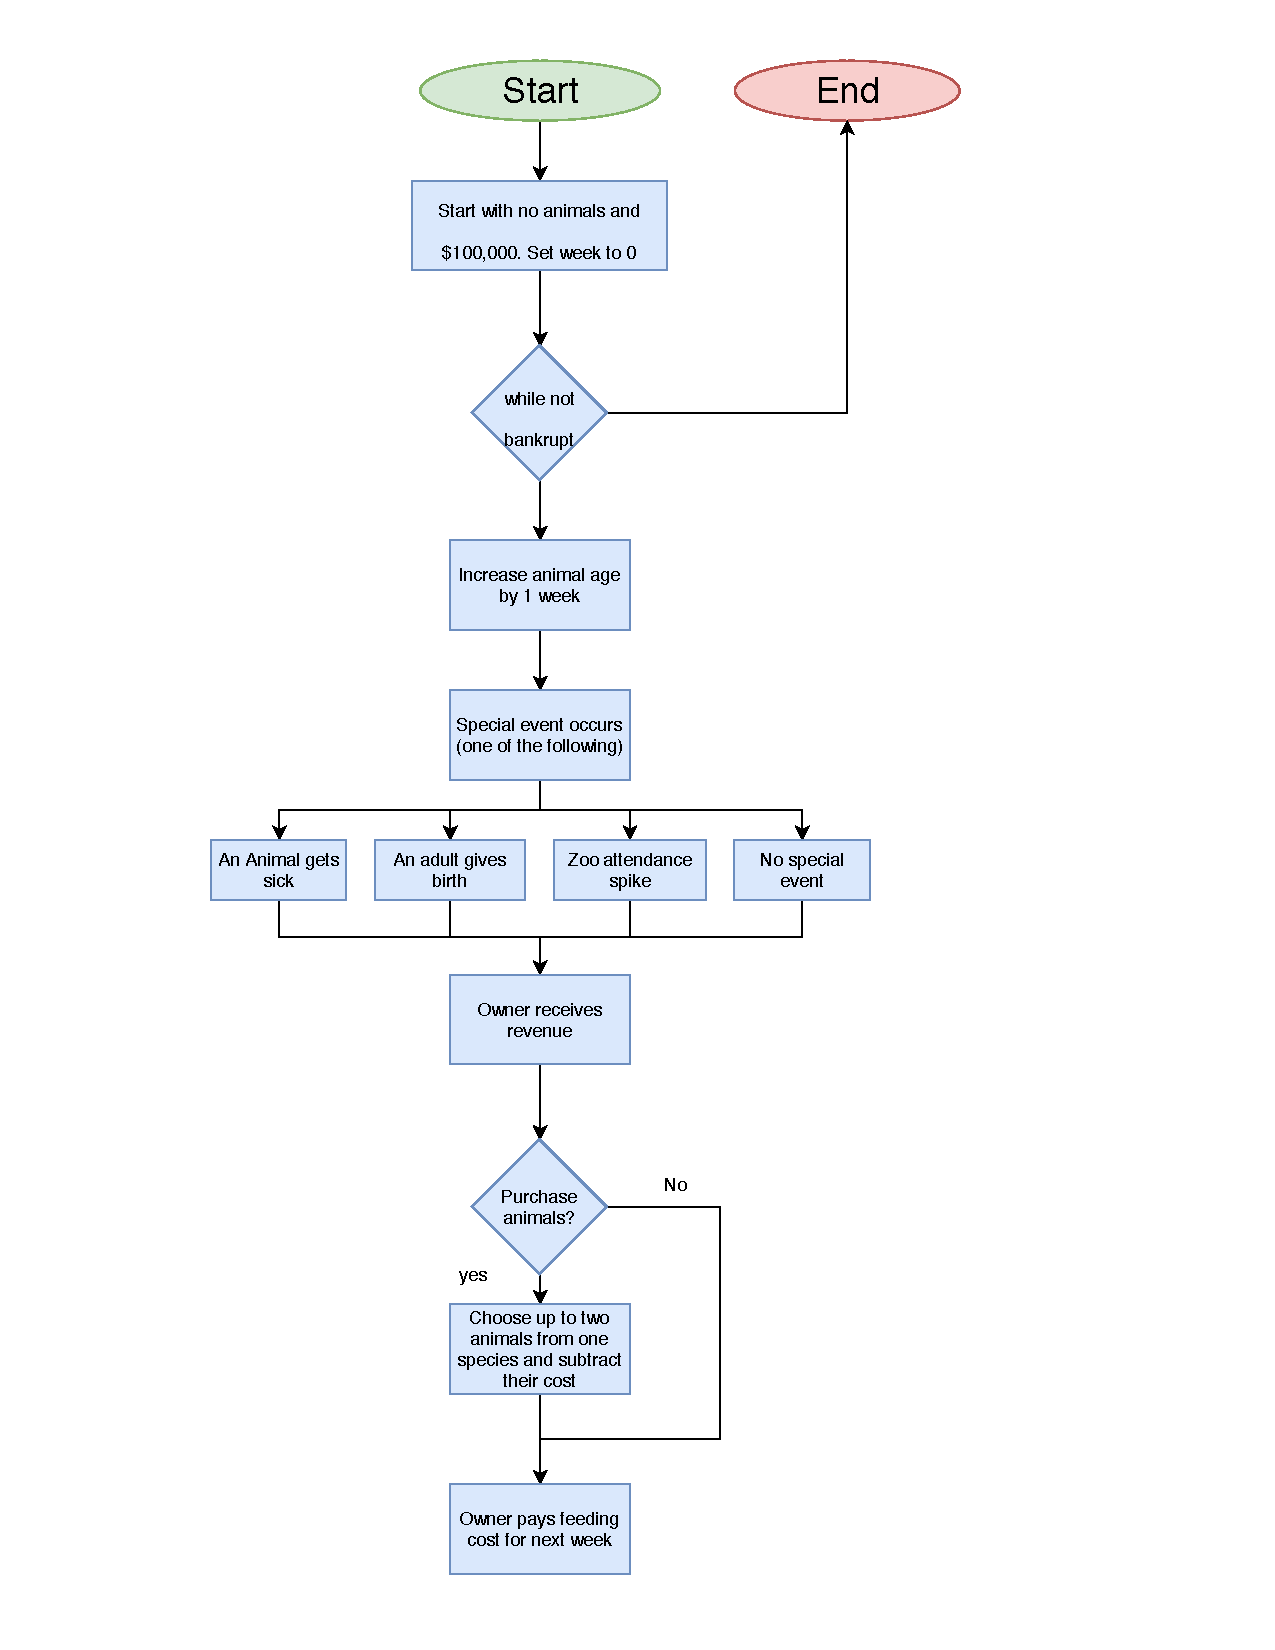
\includepdf{images/hw3_program_design.pdf}
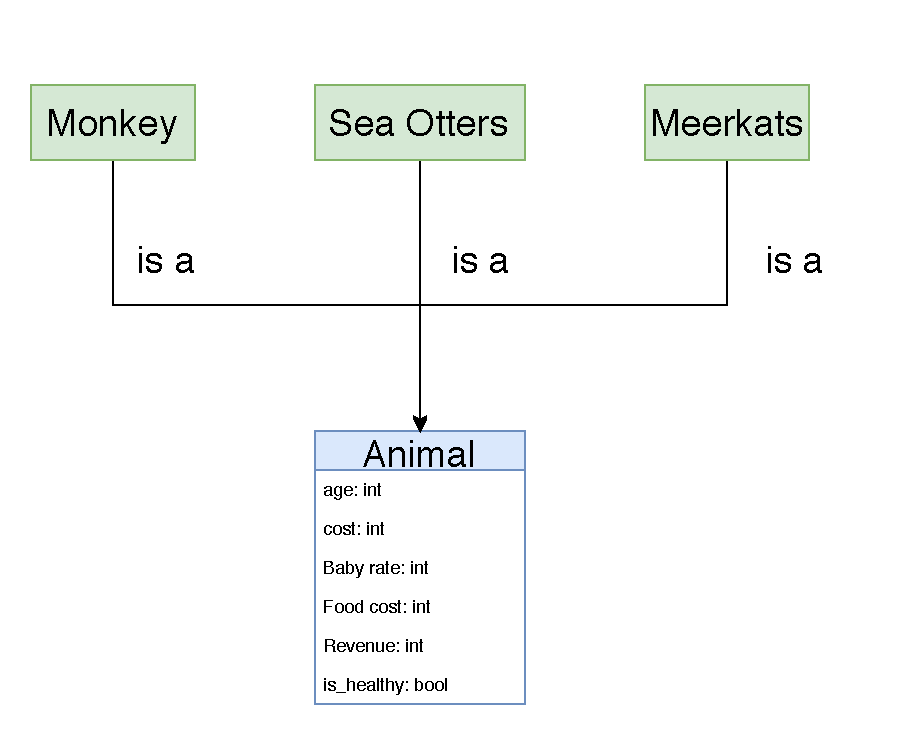
\includepdf{images/hw3_class_design.pdf}


\section*{Looking back / testing}

\textit{This includes any checking/self-reflection you did while solving the
  problem, which includes using a calculator to make sure the output is correct,
  testing to make sure your code executes correctly and behaves the way you
  expect under specific circumstances, using sources of information to make
  sense of the results, etc. However, you need to think about the input prior to
  implementation!!!}\\
\vspace{5em}

\begin{center}
 \begin{tabular}{l|l} % <-- Alignments: 1st column left, 2nd middle and 3rd right, with vertical lines in between
   \textbf{Input} & \textbf{Expected} \\
    &    \\
   \hline
   animal gets sick & animals ``is\_healthy'' attribute set to false \\
   animal gets sick and don't have enough money & animal dies and is removed from  zoo\\
   animal gets sick and do have enough money & half of animal's cost subtracted from bank\\
   addult gives birth & two new animals are added to zoo with age set to zero \\
   zoo attendance spike & revenue for monkeys increases \\
   owner runs out of money & simulation ends.
 \end{tabular}
\end{center} 






\end{document}





































